\documentclass[a4paper,11pt,fleqn]{article}

\usepackage[utf8]{inputenc}
%\usepackage[swedish]{babel}
\usepackage[lighttt]{lmodern}

%\usepackage{amsmath}
%\usepackage{amssymb}
%\usepackage{amsthm}
%\usepackage{listings}
%\usepackage{parskip}
%\usepackage{enumerate}
%\usepackage{tikz}
\usepackage{graphicx}


%\usepackage{geometry}
%\geometry{
%	%top=1.5in,
%	bottom=1.5in
%}

\author{Andreas Hagesjö \and Daniel Pettersson \and
Magnus Hagmar \and Niclas Ogeryd \and Robert Nyquist}

\title{Modell över Sveriges primärenergitillförsel \\ Kurs ENM155} 


\begin{document}
\pagenumbering{gobble} 
\maketitle
\newpage
\pagenumbering{arabic} 

\section{Introduktion}
Denna rapport innehåller en enkel modell utav Sveriges energisystem som det ser ut idag.
Modellen visar hur olika primäreneriger födelas på de tre sektorerna industri, transport och bostäder samt en uppskattning utav Sveriges totala primärenergitillförsel.


\section{Metod}
Modellen är nerbruten i tre delar, industri, transport och bostäder som är de olika sektorerna.
För varje sektor så listas alla primärenergier som birdrar till respektive sektor. Varje primärenergi går sedan vidare till de olika sekundärenergierna som den bidrar till. Varje sekundärenergi går vidare till sektorn, alternativ till en ny sekundärenergi som i sin tur går vidare till en sektor eller ytterligare en sekundärenergi. \\
I Appendix B finns de matematiska formlerna för att räkna ut primarenergierna för varje enskild sektor.


\begin{itemize}
\item Då vi har brutit ner modellen i sektorer så följer de inte diagrammet i Figur 1 i lab PM.
Istället så ger flödesschemat i Appendix A en direkt bild utav strukturen på våran implementation.


\item Modellen är byggd så att det går att ta reda på tillförseln av varje enskild primärenergi samt vilka typer av primärenergi, och mängedn, varje enskild sektor använder.
Det går även att räkna ut värden på sekundärenergierna för varje sektor med hjälp av modellen.

\item Då varje sektor innehåller alla primärenergier och sekundärenergier som bidrar så blir det väldigt enkelt att addera nya energier.
Den nya energin läggs till i sektorn den bidrar till och går sedan vidare till en sekundärenerig eller sektorn.
\end{itemize}

\newpage

\section{Resultat}

I tabbel \ref{resultat} visas den totala energitillförsel samt varje enskild energikällas tillförsel.
\begin{table}[h!]
	\centering
	\begin{tabular}{||c c||}
		\hline
		Energikälla & Tillförsel \\
		\hline
		\hline
		Biobränsle & \\
		Fossila bränslen & \\
		Vindkraft & \\
		Vattenkraft & \\
		Kärnkraft & \\
		Spillvärme & \\
		\hline
		\hline
		Totalt & \\
		\hline
	\end{tabular}
	\caption{Resultat}
	\label{resultat}
\end{table}

Presentera Sveriges totala primärenergitillförsel, samt uppdelat på
respektive energikälla.

\appendix
\section{Flödesschema}
\begin{figure}[h!]
	\centering 
 		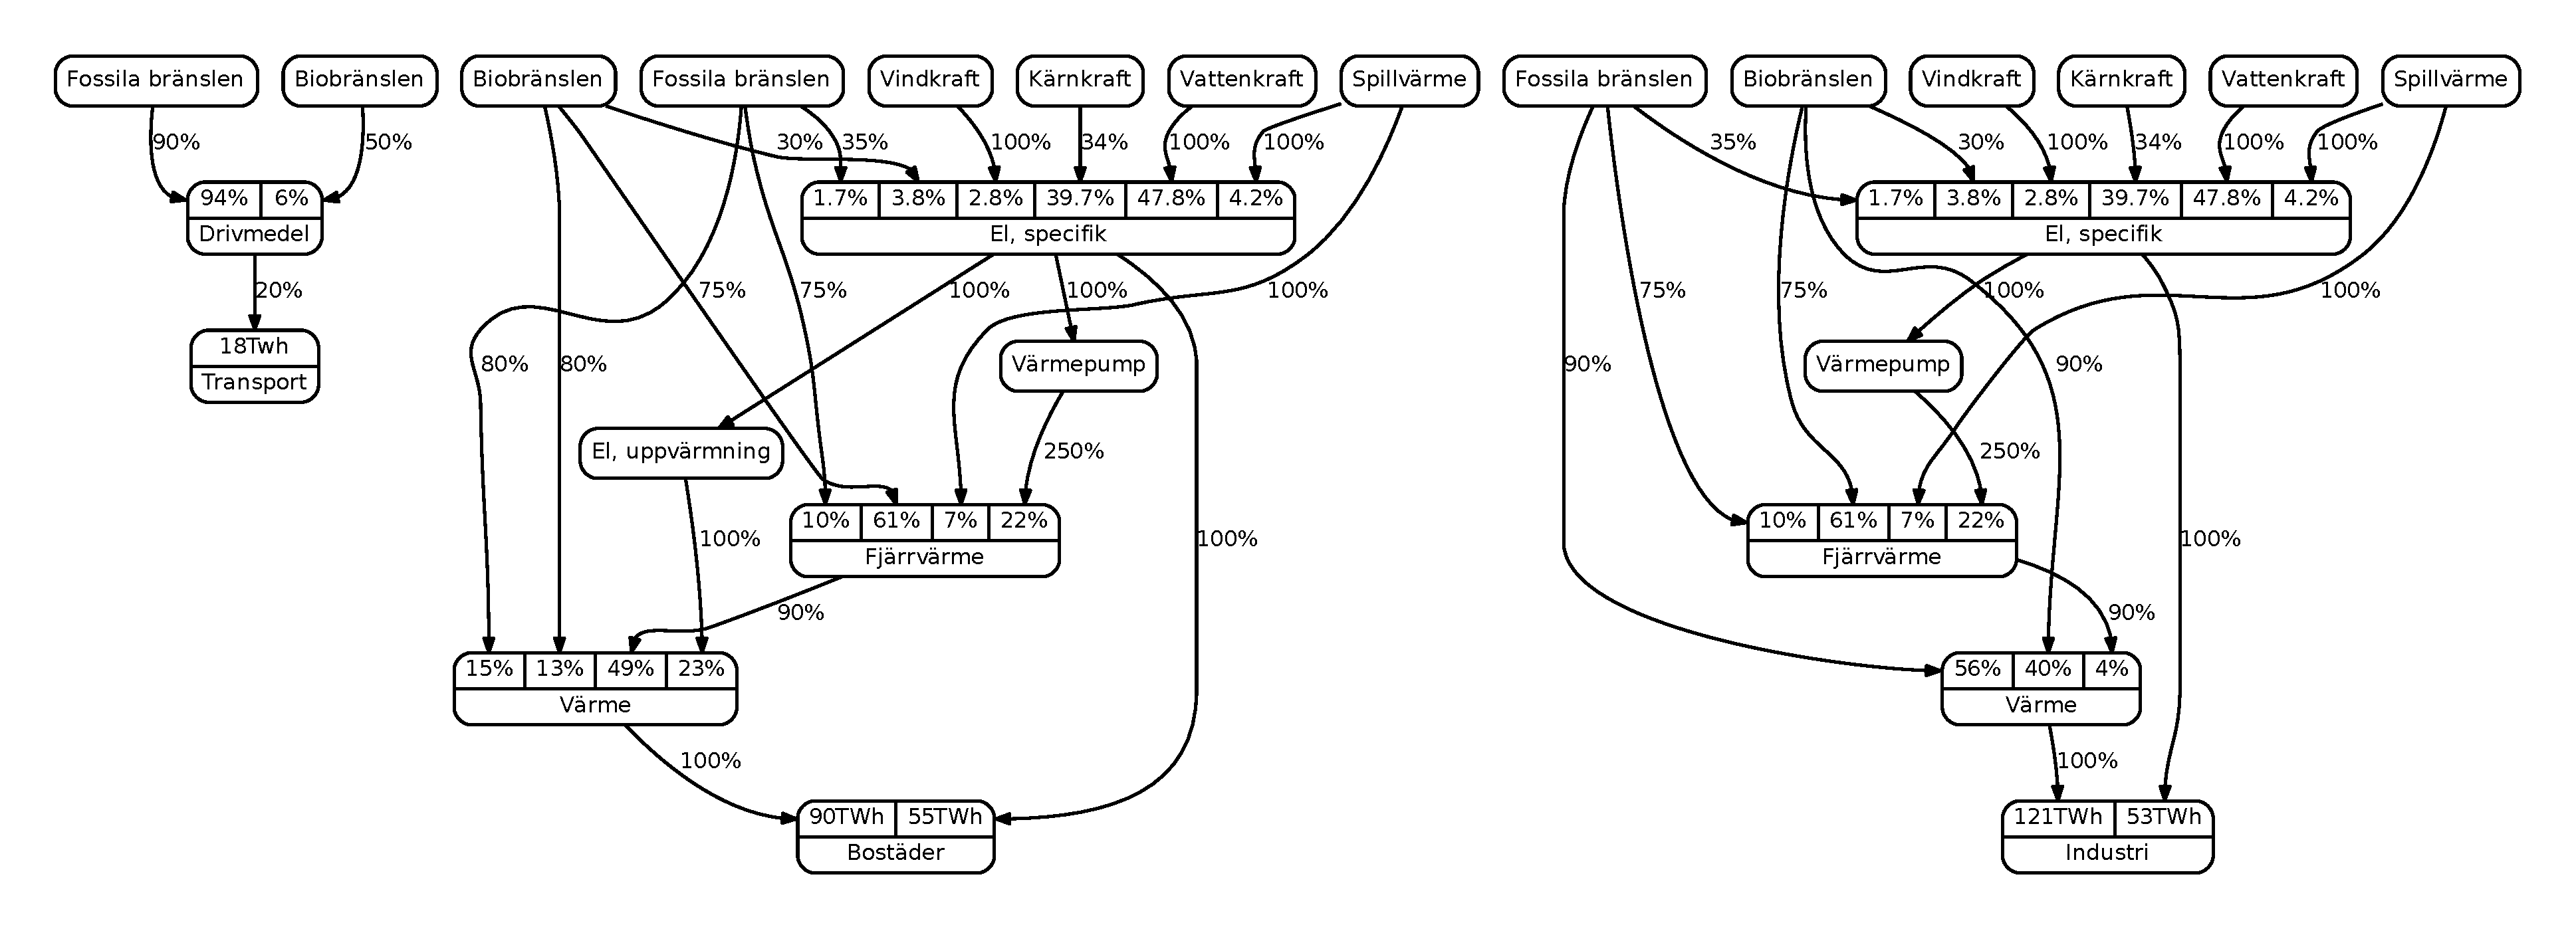
\includegraphics[scale = 0.2]{diagram.pdf}
		\label{diagram}
\end{figure}
\section {Matematisk modell}
\subsection{Transport}
\begin{figure}[h!]
	\centering 
 		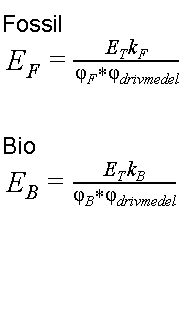
\includegraphics[scale = 0.75]{transport2.pdf}
		\label{diagram}
\end{figure}
\subsection{Bostäder}
\begin{figure}[h!]
	\centering 
 		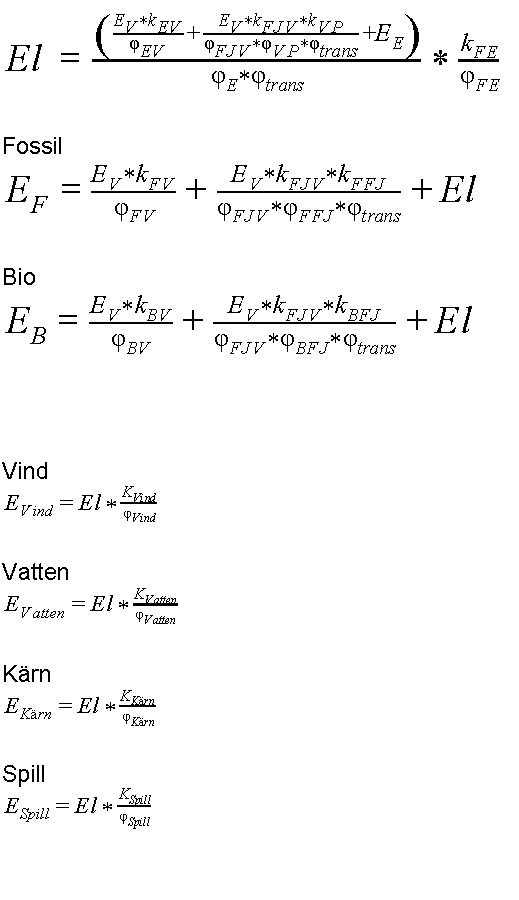
\includegraphics[scale = 0.75]{homes2.pdf}
		\label{diagram}
\end{figure}
\subsection{Industri}
\begin{figure}[h!]
	\centering 
 		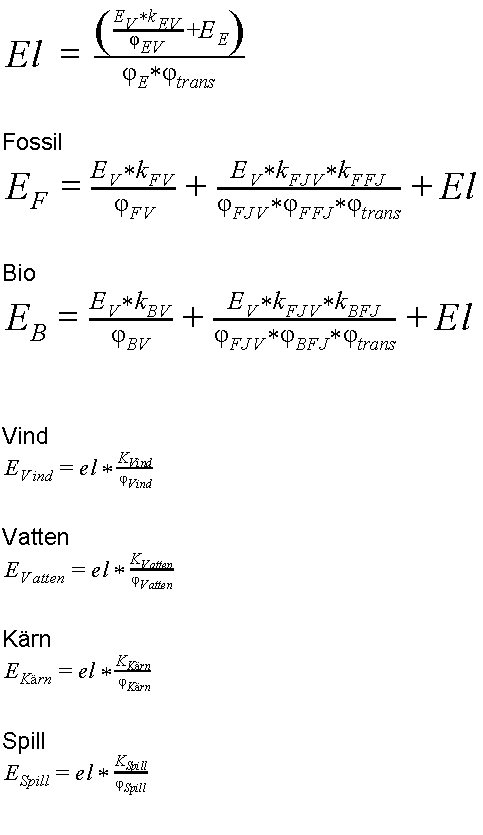
\includegraphics[scale = 0.75]{industri2.pdf}
		\label{diagram}
\end{figure}
\section{Programkod}
Bifoga koden

\end{document}

